% !TeX root = dissertation.tex
\clearpage
\onecolumn
\setcounter{table}{0}
\setcounter{figure}{0}
\renewcommand{\thetable}{A\arabic{table}}
\renewcommand{\thefigure}{A\arabic{figure}} 

%\vspace{-15pt}
%\section{Appendix}
% \label{sec:appendix}



%\begin{table}[h]
%\centering
%
%\caption{Study Questionnaire.}
%\label{tab:questionnaire}       
%
%\newcolumntype{P}[1]{>{\arraybackslash}p{#1}}
%\begin{tabular}{m{2cm}m{14cm}}
%\hline\noalign{\smallskip}
% & \multicolumn{1}{c}{Privacy-related attitude questions (7pt scale)} \\
%\noalign{\smallskip}\cmidrule(r){2-2}
%\noalign{\smallskip}
%
%\multirow{4}{*}{Trust}
%& I believe the company providing this fitness tracker is trustworthy in handling my information.\\
%& I believe this company tells the truth and fulfills promises related to the information I provide.\\
%& I believe this company is predictable and consistent regarding the usage of my information.\\
%& I believe this company is honest when it comes to using the information I provide.\\
%\cmidrule(r){2-2}
%
%\multirow{6}{2cm}{General privacy concerns}
%& All things considered, the Internet causes serious privacy problems.\\
%& Compared to others, I am more sensitive about the way online companies handle my personal information.\\
%& To me, it is the most important thing to keep my privacy intact from online companies.\\
%& I believe other people are too concerned with online privacy issues.\\
%& Compared with other subjects on my mind, personal privacy is very important.\\
%& I am concerned about threats to my personal privacy today. \\
%\cmidrule(r){2-2}
%
%\multirow{3}{2cm}{Perceived surveillance}
%& I believe that the location of my mobile device is monitored at least part of the time.\\
%& I am concerned that mobile apps are collecting too much information about me.\\
%& I am concerned that mobile apps may monitor my activities on my mobile device.\\
%\cmidrule(r){2-2}
%
%\multirow{3}{2cm}{Perceived intrusion}
%& I feel that as a result of my using mobile apps, others know about me more than I am comfortable with.\\
%& I believe that as a result of my using mobile apps, information about me that I consider private is now more readily available to others than I would want.\\
%& I feel that as a result of my using mobile apps, information about me is out there that, if used, will invade my privacy.\\
%
%\cmidrule(r){2-2}
%
%
%\multirow{3}{2cm}{Perceived secondary use of personal information}
%& I am concerned that mobile apps may use my personal information for other purposes without notifying me or getting my authorization.\\
%& When I give personal information to use mobile apps, I am concerned that apps may use my information for other purposes.\\
%& I am concerned that mobile apps may share my personal information with other entities without getting my authorization.\\
%\hline
%
% & \multicolumn{1}{c}{Negotiability of privacy settings questions (Y|N for each permission setting)} \\
% \cmidrule(r){2-2}
%& Would you share the following data if the risks significantly increased?\\
%& Would you share the following data if the benefits significantly decreased?\\
%& Would you share the following data if the risks significantly decreased?\\
%& Would you share the following data if the benefits significantly increased?\\
%\hline
%
% & \multicolumn{1}{c}{Social behaviour questions (7pt scale)} \\
%\cmidrule(r){2-2}
%\multirow{2}{2cm}{Social influence}
%& If your friends exercise, does this influence you to exercise?\\
%& If your social media friends exercise, does this influence you to exercise?\\
%\cmidrule(r){2-2}
%
%\multirow{2}{2cm}{Sociability}
%& How often do you meet new friends while you exercise?\\
%& Are you open to the idea of meeting new friends while you exercise?\\
%\hline
%
%& \multicolumn{1}{c}{Exercise tendencies questions (7pt scale; multiple choice for What questions)} \\
%\cmidrule(r){2-2}
%
%\multirow{7}{2cm}{Exercise attitude}
%& How physically healthy are you?\\
%& How important is exercise to you?\\
%& What do you most often do for exercise?\\
%& How often do you exercise?\\
%& At what intensity do you work out?\\
%& Do you feel you get too much, the right amount, or too little exercise?\\
%& What is the main reason you exercise?\\
%\cmidrule(r){2-2}
%
%\multirow{4}{2cm}{Healthy living expertise}
%& I understand difference between different types of healthy-living measures.\\
%& I know healthy-living measures that most others haven’t even heard of.\\
%& I know which healthy-living measures are useful to implement.\\
%& I am able to choose the right healthy-living measures.\\
%
%\noalign{\smallskip}\hline
%\end{tabular}
%\end{table}












\begin{table*}
\scriptsize 
\centering
% table caption is above the table
\caption{Table of Accuracies.}
\label{tab:allaccuracy}       % Give a unique label
% For LaTeX tables use
\newcolumntype{P}[1]{>{\arraybackslash}p{#1}}
\begin{tabular}{P{2.5cm}P{1.7cm}P{1.6cm}P{1.5cm}P{1.5cm}P{1.5cm}P{1.9cm}}
\hline\noalign{\smallskip}
 %& \multicolumn{2}{c}{Baseline}  %\parbox{2.5cm}{Pick Profile\\ (Upper Bound)}
%  & Pick Profile (UB)  &  Single Smart Default (LB) & Direct questions & Privacy Attitude & Homophily Effect & Negotiability \\
 & Pick Profile &  Single Smart Default & Direct prediction & Privacy Attitude & Social Behaviour & Negotiability \\
\noalign{\smallskip}\cmidrule(r){2-7}\noalign{\smallskip}



\textit{S Set}\\
\\
Identity & 66.67 \% & 66.67 \% &66.67 \%  & 66.67 \% &  66.67 \% & 66.67 \%\\
Contacts & 83.33 \% & 70.00 \% &70.00 \% & 56.67 \% & 73.33 \% & 80.00 \%\\
Location & 83.33 \% & 83.33 \% &83.33 \% &  83.33 \% & 83.33 \% & 83.33 \%\\
SMS  & 90.00 \% & 50.00 \% & 70.00 \% & 50.00 \% & 53.33 \% & 73.33 \%\\
Storage & 83.33 \% & 56.67 \% &70.00 \%  & 43.33 \% & 46.67 \%& 60.00 \%\\
Camera  & 80.00 \% & 60.00 \% &86.67 \%  & 60.00 \% & 70.00 \% & 63.33 \%\\
Bluetooth & 83.33 \% & 83.33 \% & 83.33 \%  & 83.33 \% & 83.33 \% & 83.33 \%\\
Photos & 80.00 \% & 66.67 \%  & 100.00 \%  & 60.00 \%  & 76.66 \% & 70.00 \%\\
Phone & 96.67 \% & 56.67 \% & 76.67 \% & 50.00 \% & 60.00 \% & 80.00 \%\\
Motion & 96.67 \% & 96.67 \% & 96.67 \% & 96.67 \% & 96.67 \% & 96.67 \%\\
Media & 70.00 \% & 76.67 \% & 56.67 \% & 43.33 \% & 33.33 \% & 60.00 \%\\
Mobile Data & 76.67 \% & 76.67 \% &76.67 \% & 76.67 \% & 76.67 \% & 76.67 \%\\

\cmidrule(r){2-7}
Average & 82.50 \%& 70.28 \% & 78.06 \% & 64.17 \% & 68.33 \% & 74.44 \%\\
\cmidrule(r){1-7}
\textit{A set}\\
\\

First Name &100.00 \% & 63.33 \% &100.00 \%& 63.33 \%& 73.33 \% & 56.67 \%\\
Last Name &96.67 \% &60.00 \% &96.67 \%& 60.00 \%& 70.00 \% & 60.00 \%\\
Gender &76.67 \% &76.67 \% & 76.67 \% & 76.67 \%& 76.67 \% & 76.67 \%\\
Birthday &90.00 \%&60.00 \% &90.00 \%  & 60.00 \% & 63.33 \%& 53.33 \%\\
Height &70.00 \% &70.00 \% & 70.00 \% & 70.00 \% & 70.00 \%& 70.00 \%\\
Weight &70.00 \% &70.00 \% & 70.00 \% & 70.00 \%& 70.00 \%& 70.00 \%\\

\cmidrule(r){2-7}
Average & 83.89 \% & 66.67 \% & 83.89 \% & 66.67\% & 70.55\% & 64.44 \%\\ 
\cmidrule(r){1-7}
\textit{F set}\\
\\
Steps & 96.67 \% & 73.33 \% &96.67 \%  & 76.67 \%& 70.00 \% & 76.67 \%\\
Distance & 96.67 \% &73.33 \% &96.67 \% & 76.67 \% & 70.00 \%& 76.67 \%\\
Elevation & 100.00 \%&70.00 \% &100.00 \% & 73.33 \% & 73.33 \%& 80.00 \%\\
Floors & 96.67 \%& 73.33 \% &96.67 \% & 76.67 \% & 70.00 \% & 76.67 \%\\
Activity minutes &100.00 \% & 70.00 \% & 100.00 \% & 73.33 \% & 73.33 \% & 80.00 \%\\
Calories activity &96.67 \%&73.33 \% &96.67 \% & 76.67 \% & 70.00 \% & 76.67 \%\\
Weight &90.00 \% &60.00 \% &90.00 \% & 63.33 \% & 70.00 \%& 76.67 \%\\
Sleep &93.33 \% &63.33 \% &93.33 \% & 66.67 \% & 66.67 \% & 80.00 \%\\
Heartrate &100.00 \% &70.00 \% &100.00 \% & 73.33 \% & 73.33 \% & 80.00 \%\\
Food logs &90.00 \% &60.00 \% &90.00 \% & 63.33 \% & 70.00 \%& 76.67 \%\\
Friends &83.33 \% &53.33 \% &83.33 \% & 56.67 \% & 63.33 \% & 70.00 \%\\
Profile &96.67 \% &66.67 \% &96.67 \% & 70.00 \% &76.67 \% & 76.67 \%\\
Location  &86.67 \% &56.67 \% &86.67 \% & 60.00 \% & 66.67 \% & 66.67 \%\\
Device \& settings &93.33 \%  & 63.33 \% &93.33 \% & 66.67 \% & 73.33 \% & 73.33 \%\\

\cmidrule(r){2-7}
Average & 94.29 \%& 66.19 \% & 94.29 \% & 69.52 \% &  70.48 \% & 76.19 \%\\
\cmidrule(r){1-7}

\textit{G set}\\
SN Public &90.00 \% &90.00 \% &90.00 \%  & 90.00 \% &90.00 \% &90.00 \%\\
SN Friends Only &73.33 \% &53.33 \% &73.33 \% & 63.33\% &60.00 \% &56.67 \%\\
Health &66.67 \% &60.00 \% &60.00 \%  & 43.33 \% &40.00 \% &70.00 \%\\
Other Apps &76.67 \% &76.67 \% &76.67 \% & 76.67 \% & 76.67 \% &76.67 \%\\
Corporate & 80.00 \% & 80.00 \% & 80.00 \% & 80.00 \% & 80.00 \% & 80.00 \%\\
Government &86.67 \% & 86.67 \% &86.67 \% & 86.67 \% & 86.67 \% &86.67 \%\\
Health &86.67 \% &86.67 \% &86.67 \% & 86.67 \% & 86.67 \% &86.67 \%\\
Safety &90.00 \% & 90.00 \% & 90.00 \%  & 90.00 \% & 90.00 \% &90.00 \%\\
Social &93.33 \% &60.00 \% &100.00 \% & 70.00 \% & 60.00 \% &63.33 \%\\
Commercial & 73.33 \% & 73.33 \% & 73.33 \% & 73.33 \% & 73.33 \%&73.33 \%\\
Convenience & 80.00 \% & 73.33 \% &73.33 \% & 76.67 \% & 66.67 \% & 70.00 \%\\
Frequency & 53.33 \% & 53.33 \% &53.33 \% & 53.00 \% & 53.33 \% & 53.33 \%\\
Retention &50.00 \% & 40.00 \% & 50.00 \% & 50.00 \% & 43.33 \% & 46.67 \%\\

\cmidrule(r){2-7}
Average & 76.92 \% & 71.02 \% & 76.41 \% & 72.31 \% & 69.74 \% & 72.56 \%\\
\cmidrule(r){1-7}
Over-all Average & 84.74 \% & 68.74 \% & 83.41 \% & 68.52 \% & 69.70 \% & 73.11 \%  \\
\end{tabular}
\end{table*}

\begin{figure}
	\centering
	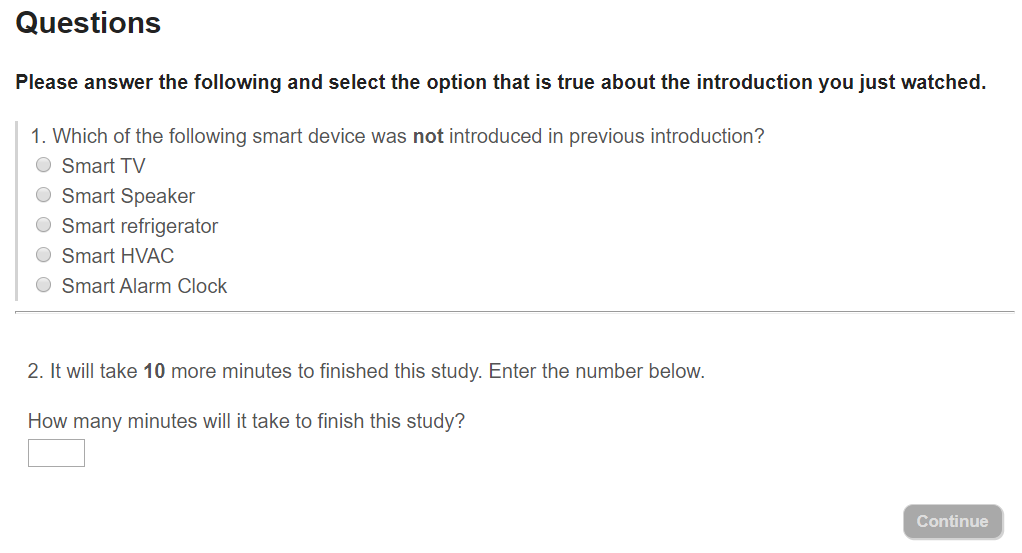
\includegraphics[width=\textwidth]{figures/yangAttentionCheck.png}
	\caption{Attention Check Question of Evaluating privacy-setting UI for Household IoT}
	\label{fig:yangAttentionCheck}
\end{figure}

\begin{figure}
	\centering
	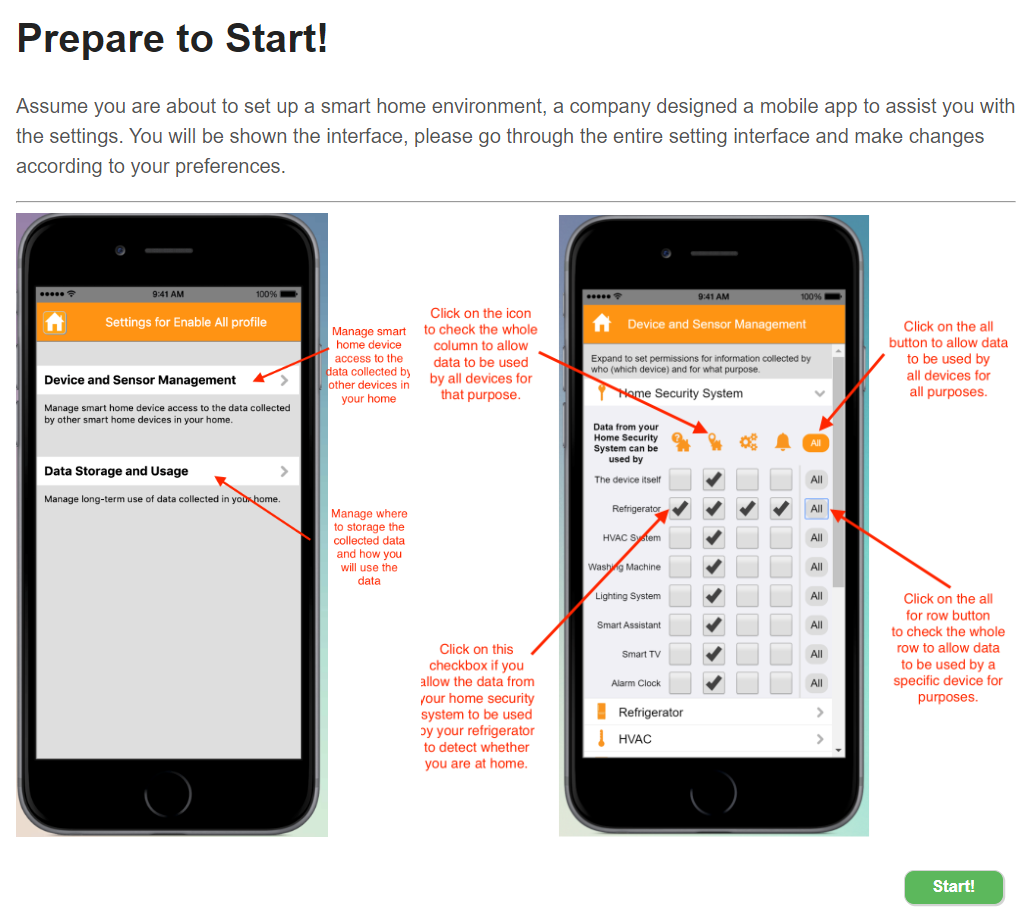
\includegraphics[width=\textwidth]{figures/yangPrepage.png}
	\caption{Instructions on how to use the UIs}
	\label{fig:yangPrepage}
\end{figure}


%ALL THE TREE VALIDATION

% \begin{figure*}
% \centering
%     \subfloat[S dataset]
% {  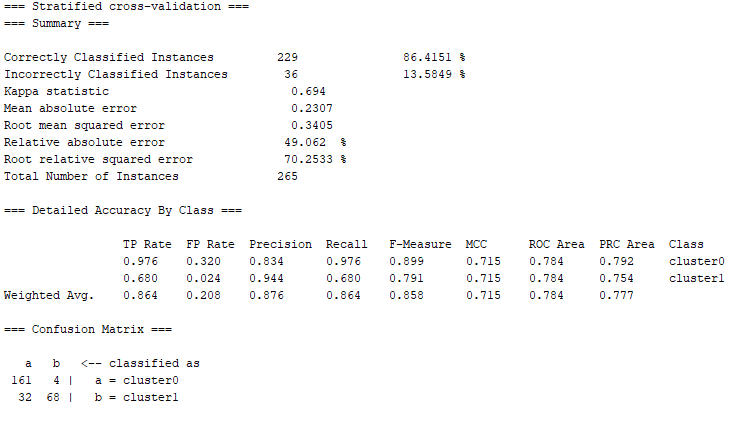
\includegraphics[width=0.67\linewidth]{figures/s_tree1sum.png}
%     \label{fig:streesum1}}
    
%     \subfloat[A dataset]
% {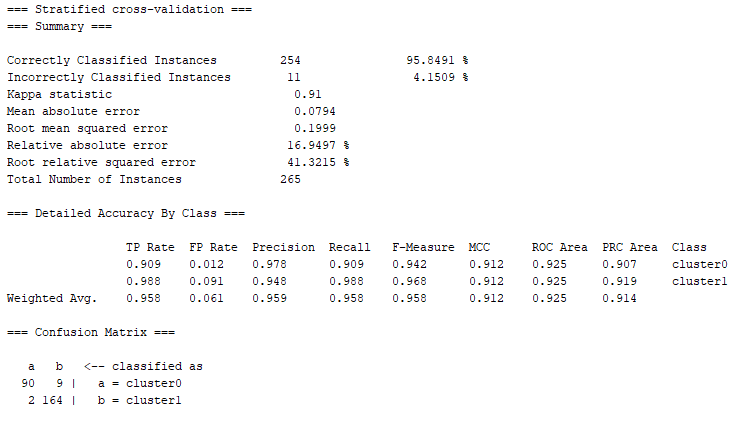
\includegraphics[width=0.67\linewidth]{figures/a_tree1sum.png}
%     \label{fig:atreesum1}}

%    \subfloat[F dataset]
% {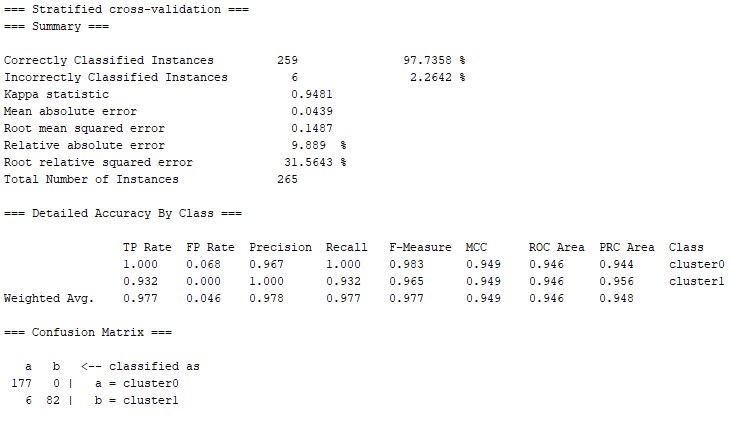
\includegraphics[width=0.67\linewidth]{figures/f_tree1sum.png}
%    \label{fig:ftreesum1}}
   
%   \subfloat[G dataset]
% {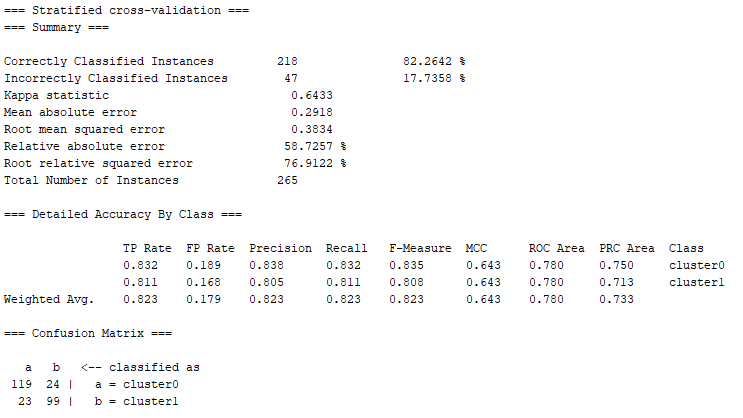
\includegraphics[width=0.67\linewidth]{figures/g_tree1sum.png}
%   \label{fig:gtreesum1}}
% \caption{The complete evaluation details for the Direct Questions.}
% \label{fig:tree1apendix}
% \end{figure*}





% \begin{figure*}
% \centering
%     \subfloat[S dataset]
% {  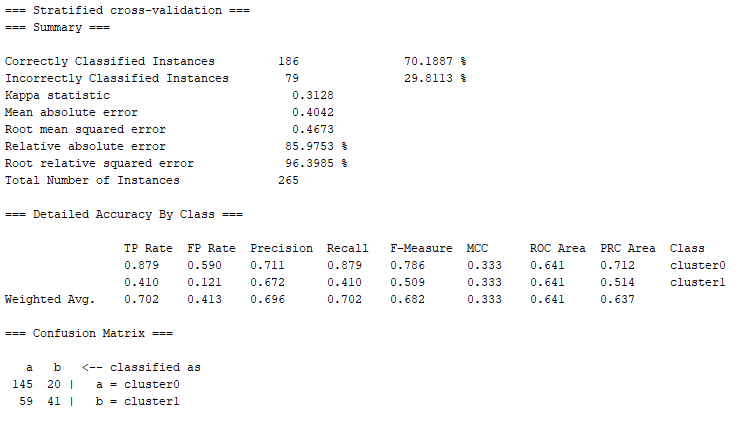
\includegraphics[width=0.67\linewidth]{figures/s_tree2sum.png}
%     \label{fig:atreesum2}}
    
%     \subfloat[S dataset]
% {  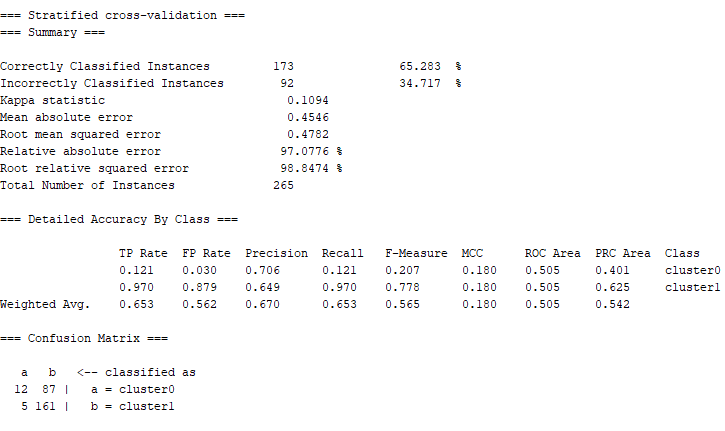
\includegraphics[width=0.67\linewidth]{figures/a_tree2sum.png}
%     \label{fig:streesum2}}
    
%     \subfloat[S dataset]
% {  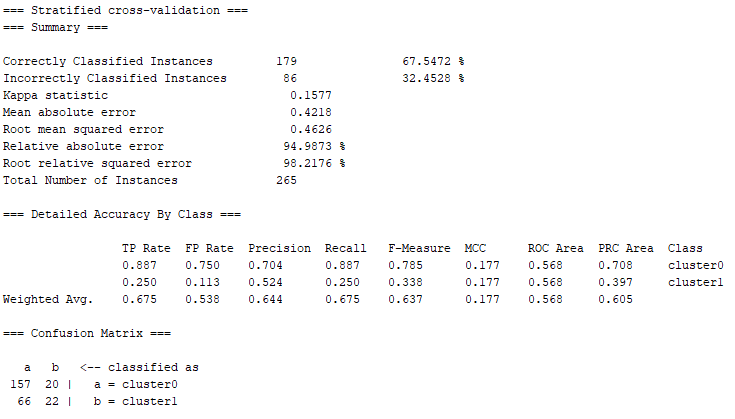
\includegraphics[width=0.67\linewidth]{figures/f_tree2sum.png}
%     \label{fig:ftreesum2}}
    
%     \subfloat[S dataset]
% {  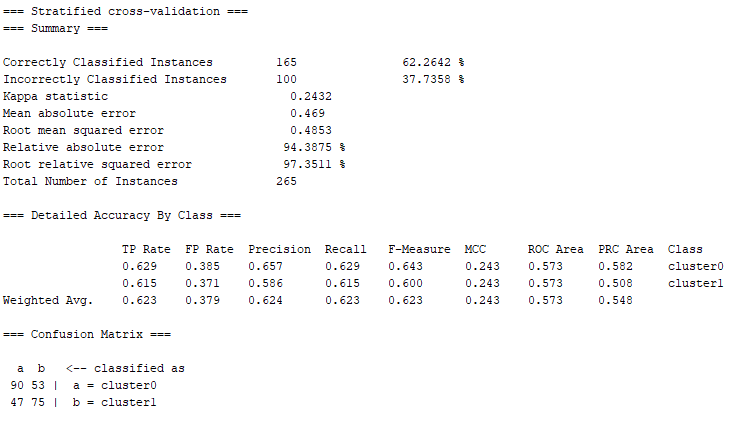
\includegraphics[width=0.67\linewidth]{figures/g_tree2sum.png}
%     \label{fig:gtreesum2}}
    
% \caption{Attitude Trees.}
% \label{fig:tree2apendix}
% \end{figure*}



% \begin{figure*}
% \centering
%     \subfloat[S dataset]
% {  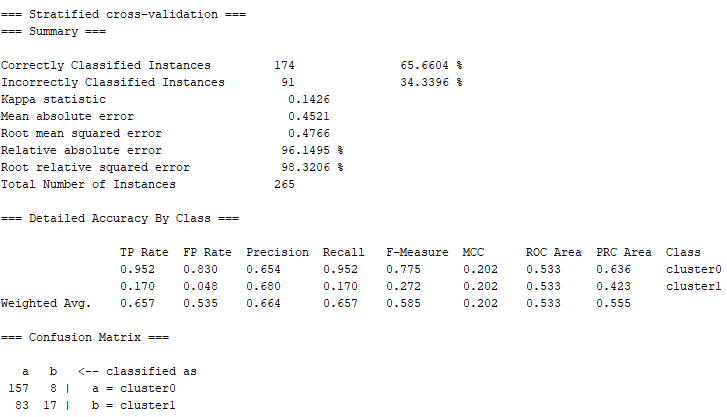
\includegraphics[width=0.67\linewidth]{figures/s_tree3sum.png}
%     \label{fig:atreesum3}}
    
%     \subfloat[S dataset]
% {  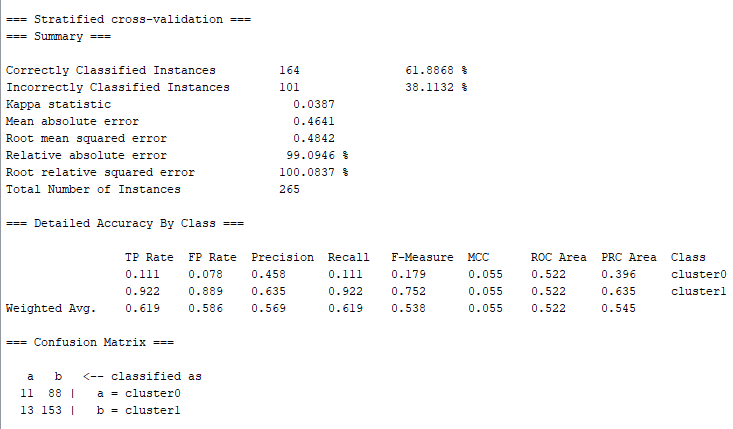
\includegraphics[width=0.67\linewidth]{figures/a_tree3sum.png}
%     \label{fig:streesum3}}
    
%     \subfloat[S dataset]
% {  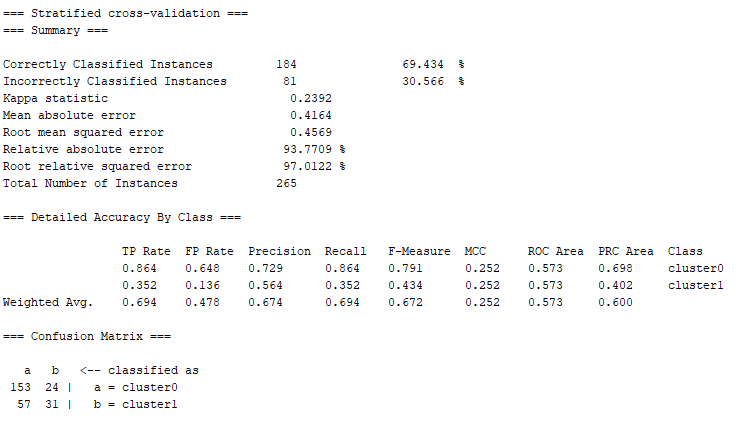
\includegraphics[width=0.67\linewidth]{figures/f_tree3sum.png}
%     \label{fig:ftreesum3}}
    
%     \subfloat[S dataset]
% {  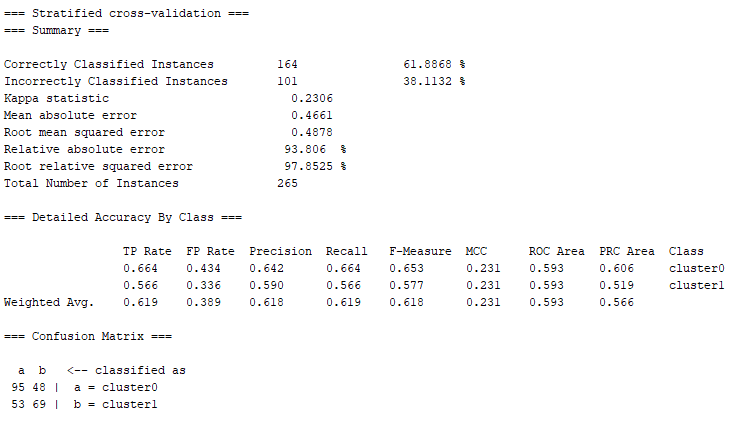
\includegraphics[width=0.67\linewidth]{figures/g_tree3sum.png}
%     \label{fig:gtreesum3}}
    
% \caption{Homophily/Social influence Trees.}
% \label{fig:tree3apendix}
% \end{figure*}

% \begin{figure*}
% \centering
%     \subfloat[S dataset]
% {  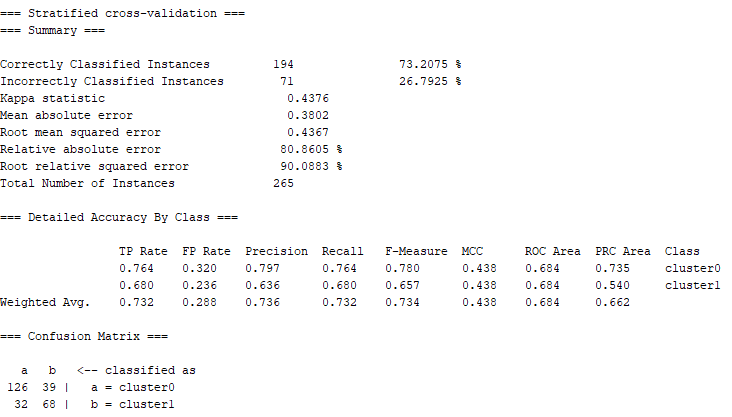
\includegraphics[width=0.67\linewidth]{figures/s_tree4sum.png}
%     \label{fig:atreesum4}}
    
%     \subfloat[S dataset]
% {  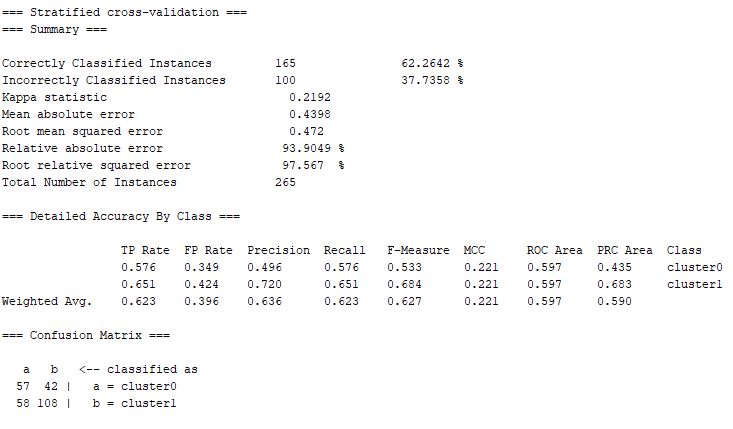
\includegraphics[width=0.67\linewidth]{figures/a_tree4sum.png}
%     \label{fig:streesum4}}
    
%     \subfloat[S dataset]
% {  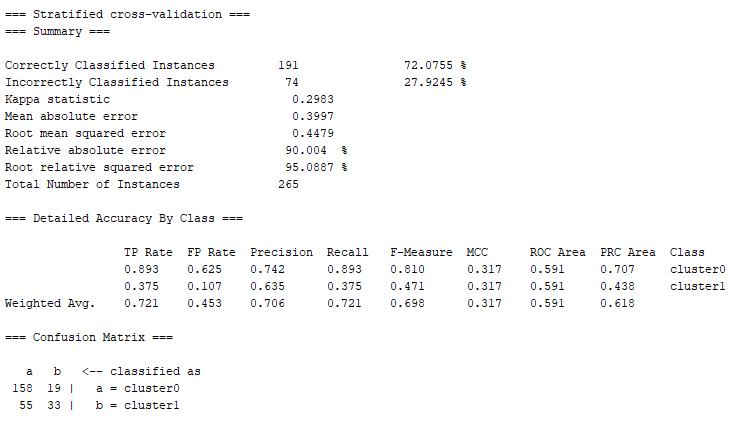
\includegraphics[width=0.67\linewidth]{figures/f_tree4sum.png}
%     \label{fig:ftreesum4}}
    
%     \subfloat[S dataset]
% {  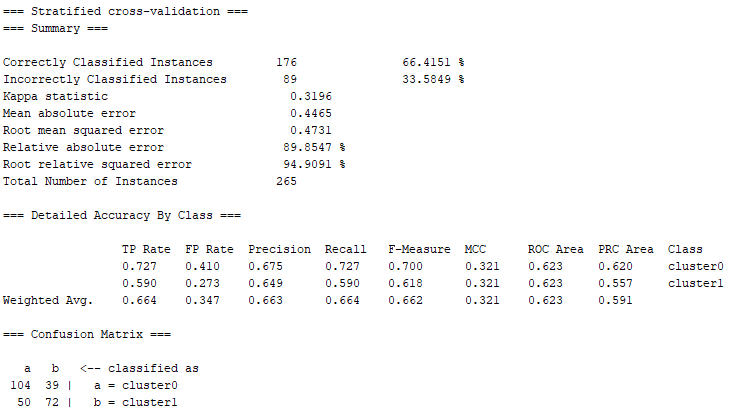
\includegraphics[width=0.67\linewidth]{figures/g_tree4sum.png}
%     \label{fig:gtreesum4}}
    
% \caption{Negotiability Trees.}
% \label{fig:tree4appendix}
% \end{figure*}

%Figure~\ref{fig:ui1AllOff} shows the experimental condition --- UI1:Everything-Off.
\begin{figure}
	\centering
	\begin{subfigure}[t]{0.24\textwidth}
		\centering
		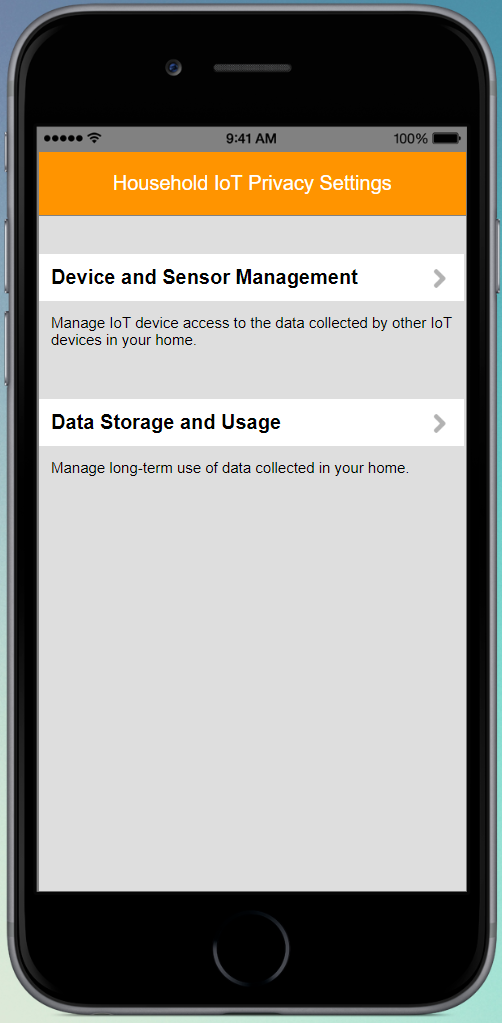
\includegraphics[height=2.8in]{figures/ui1allOff1.png}
	\end{subfigure}%
	~
	\begin{subfigure}[t]{0.24\textwidth}
		\centering
		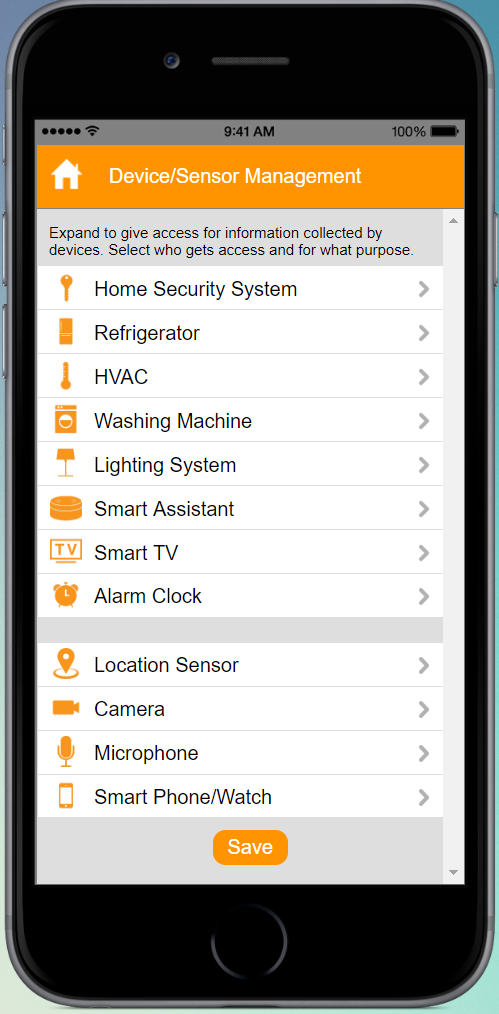
\includegraphics[height=2.8in]{figures/ui1allOff2.png}
	\end{subfigure}%
	~
	\begin{subfigure}[t]{0.24\textwidth}
		\centering
		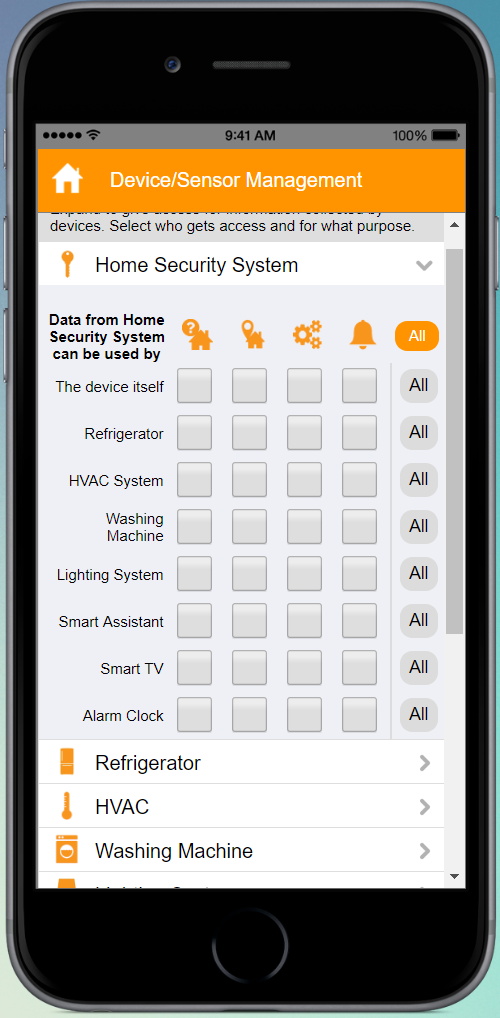
\includegraphics[height=2.8in]{figures/ui2allOff3.png}
	\end{subfigure}%
	~
	\begin{subfigure}[t]{0.24\textwidth}
		\centering
		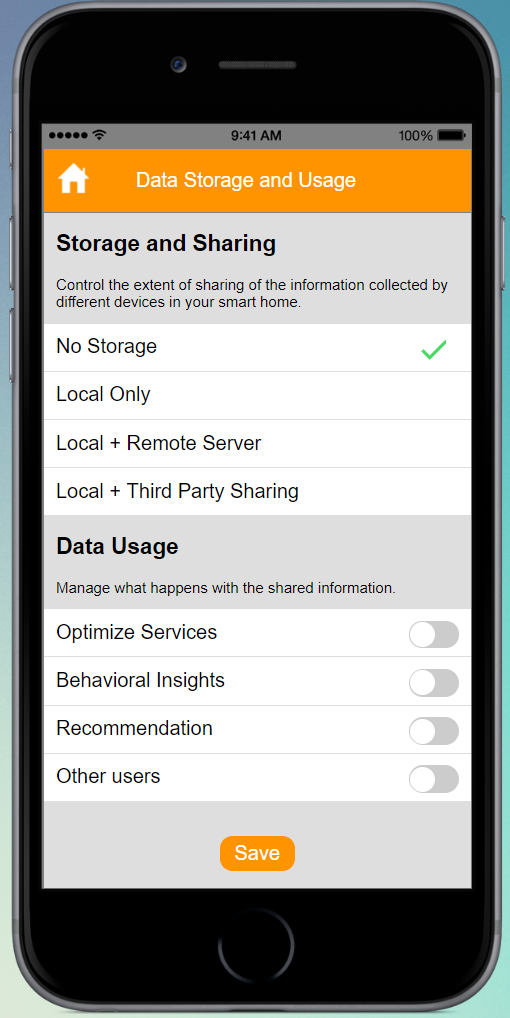
\includegraphics[height=2.8in]{figures/ui1allOff4.png}
	\end{subfigure}%
	\caption{User Interface 1 with all settings turned off}
	\label{fig:ui1AllOff}
\end{figure}

%Figure~\ref{fig:ui2AllOff} shows the experimental condition --- UI2:Everything-Off.
\begin{figure}
	\centering
	\begin{subfigure}[t]{0.2\textwidth}
		\centering
		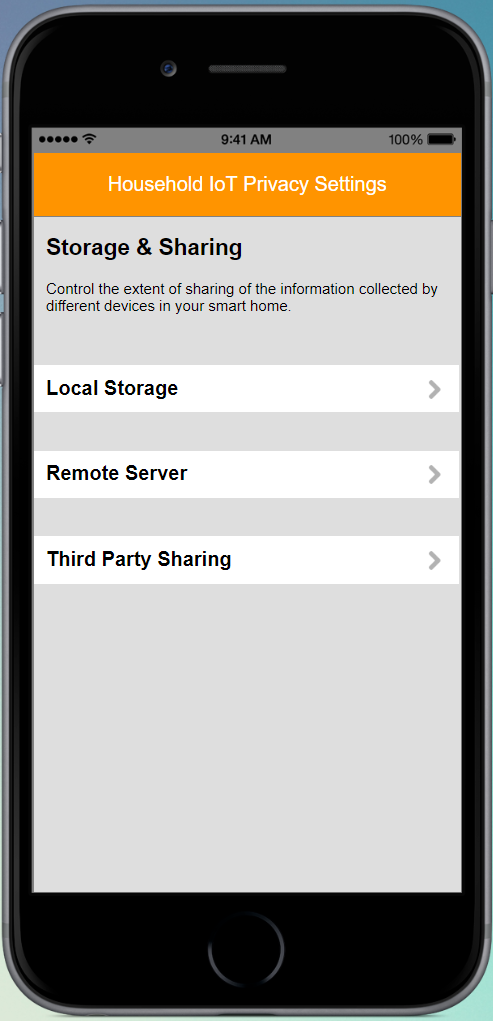
\includegraphics[height=2.8in]{figures/ui2allOff1.png}
	\end{subfigure}%
	~~~~~
	\begin{subfigure}[t]{0.2\textwidth}
		\centering
		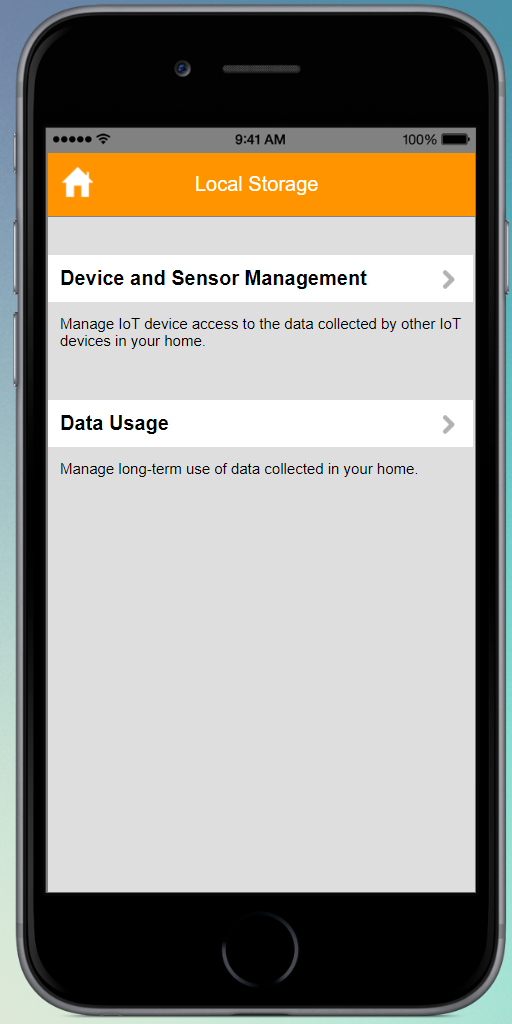
\includegraphics[height=2.8in]{figures/ui2allOffLocal.png}
	\end{subfigure}%
	~~~~~
	\begin{subfigure}[t]{0.2\textwidth}
		\centering
		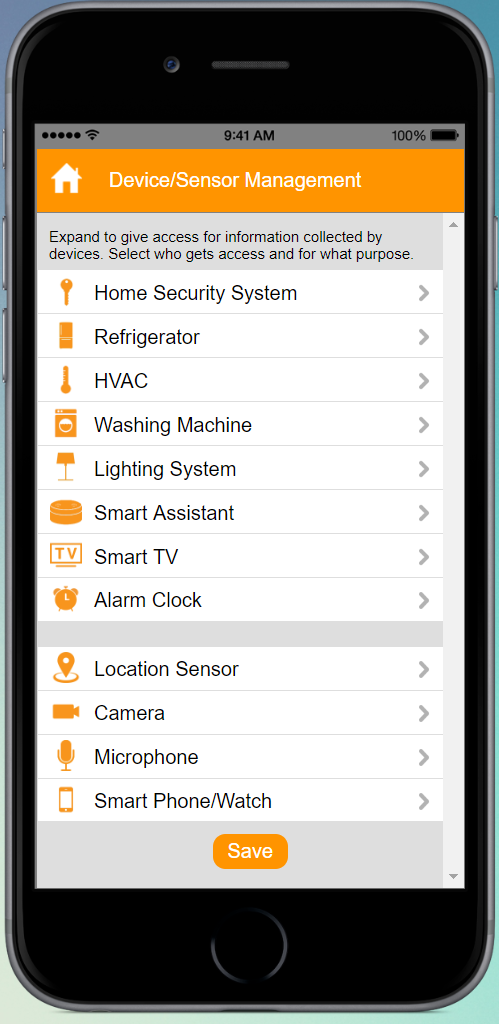
\includegraphics[height=2.8in]{figures/ui2allOff2.png}
	\end{subfigure}%
	~~~~~
	\begin{subfigure}[t]{0.2\textwidth}
		\centering
		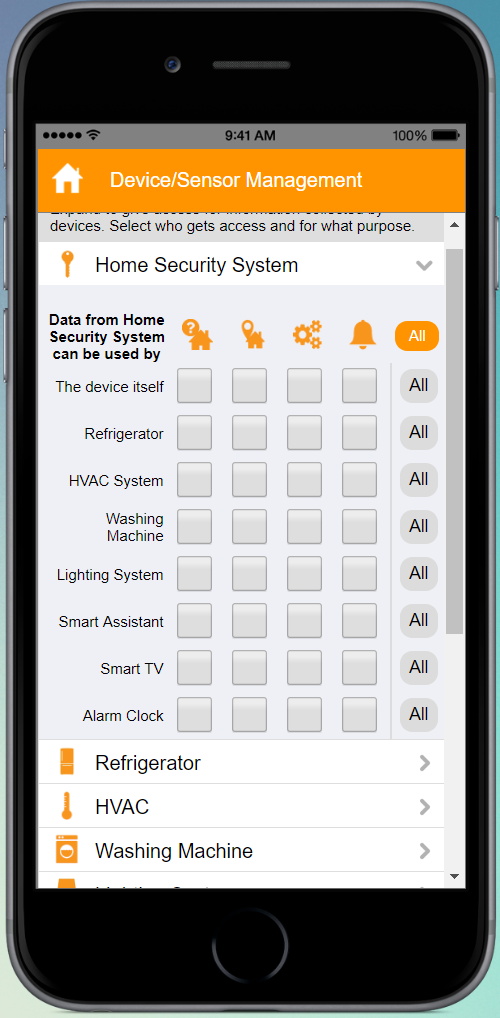
\includegraphics[height=2.8in]{figures/ui2allOff3.png}
	\end{subfigure}%
	~~~~~
	\begin{subfigure}[t]{0.2\textwidth}
		\centering
		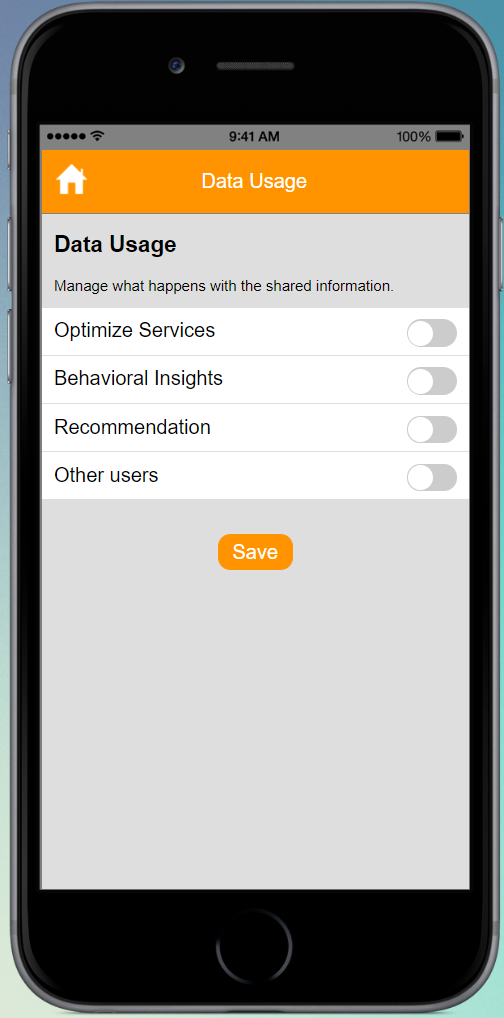
\includegraphics[height=2.8in]{figures/ui2allOff4.png}
	\end{subfigure}%
	\caption{User Interface 2 with all settings turned off}
	\label{fig:ui2AllOff}
\end{figure}

%Figure~\ref{fig:ui1AllOn} shows the experimental condition --- UI1:Everything-On.
\begin{figure}
	\centering
	\begin{subfigure}[t]{0.24\textwidth}
		\centering
		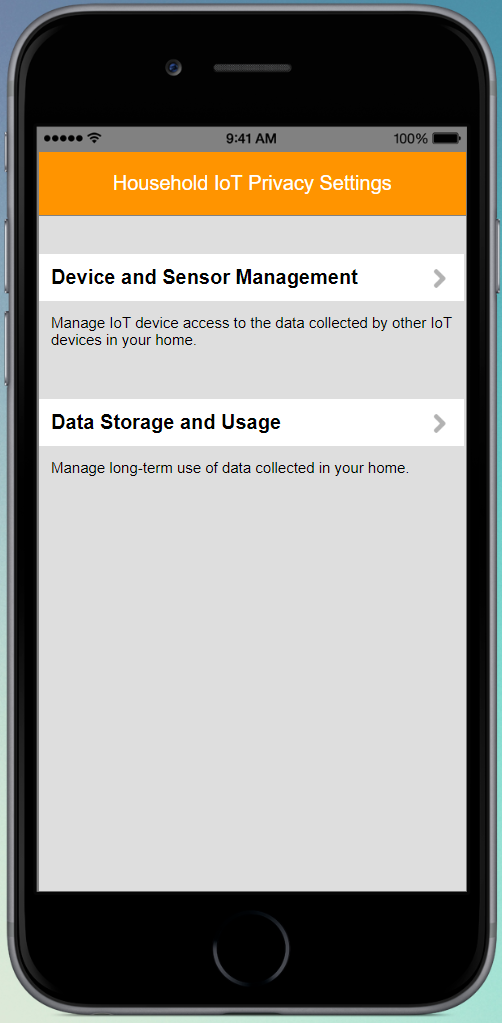
\includegraphics[height=2.8in]{figures/ui1allOff1.png}
	\end{subfigure}%
	~
	\begin{subfigure}[t]{0.24\textwidth}
		\centering
		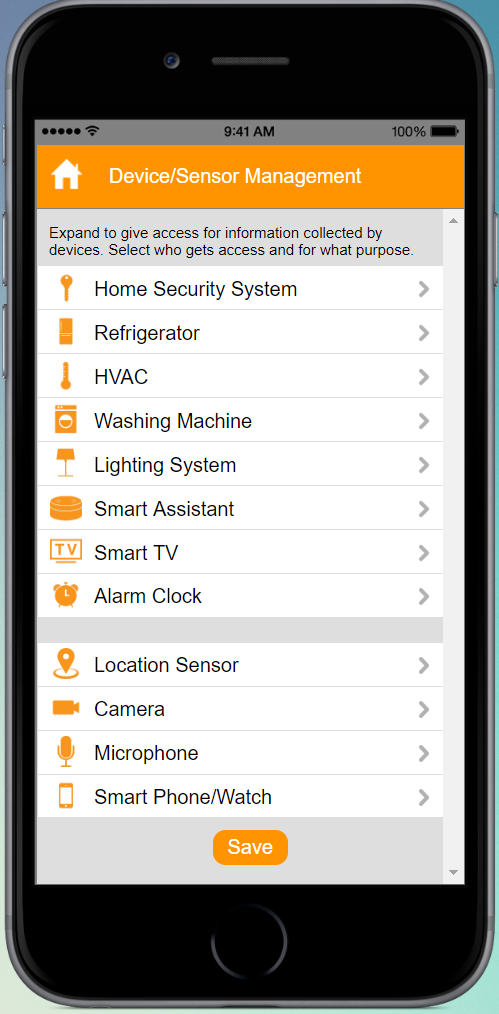
\includegraphics[height=2.8in]{figures/ui1allOff2.png}
	\end{subfigure}%
	~
	\begin{subfigure}[t]{0.24\textwidth}
		\centering
		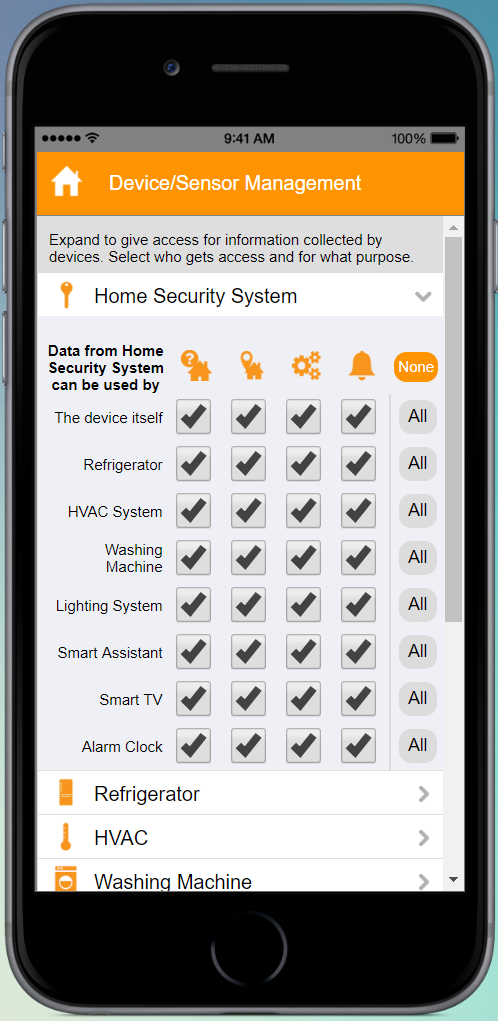
\includegraphics[height=2.8in]{figures/ui2allOn3.png}
	\end{subfigure}%
	~
	\begin{subfigure}[t]{0.24\textwidth}
		\centering
		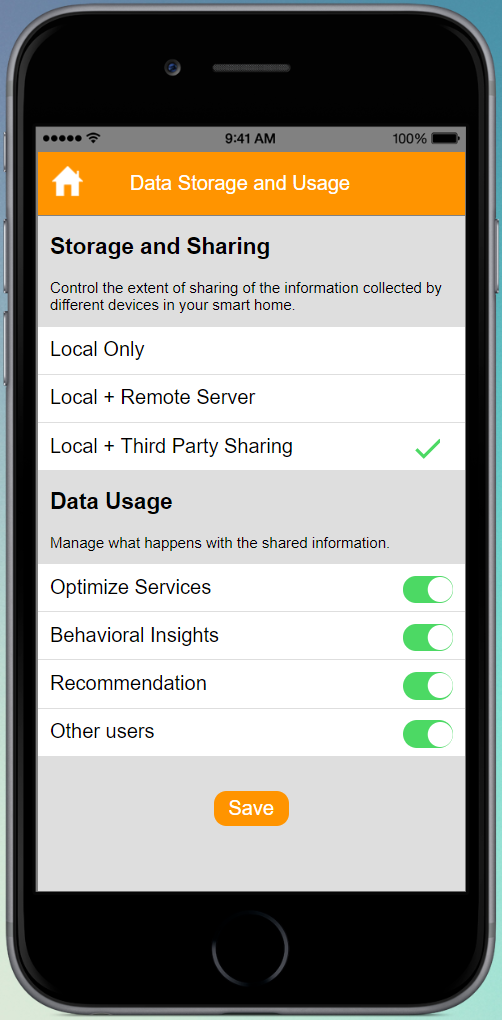
\includegraphics[height=2.8in]{figures/ui1allOn4.png}
	\end{subfigure}%
	\caption{User Interface 1 with all settings turned on}
	\label{fig:ui1AllOn}
\end{figure}

%Figure~\ref{fig:ui2AllOn} shows the experimental condition --- UI2:Everything-On.
\begin{figure}
	\centering
	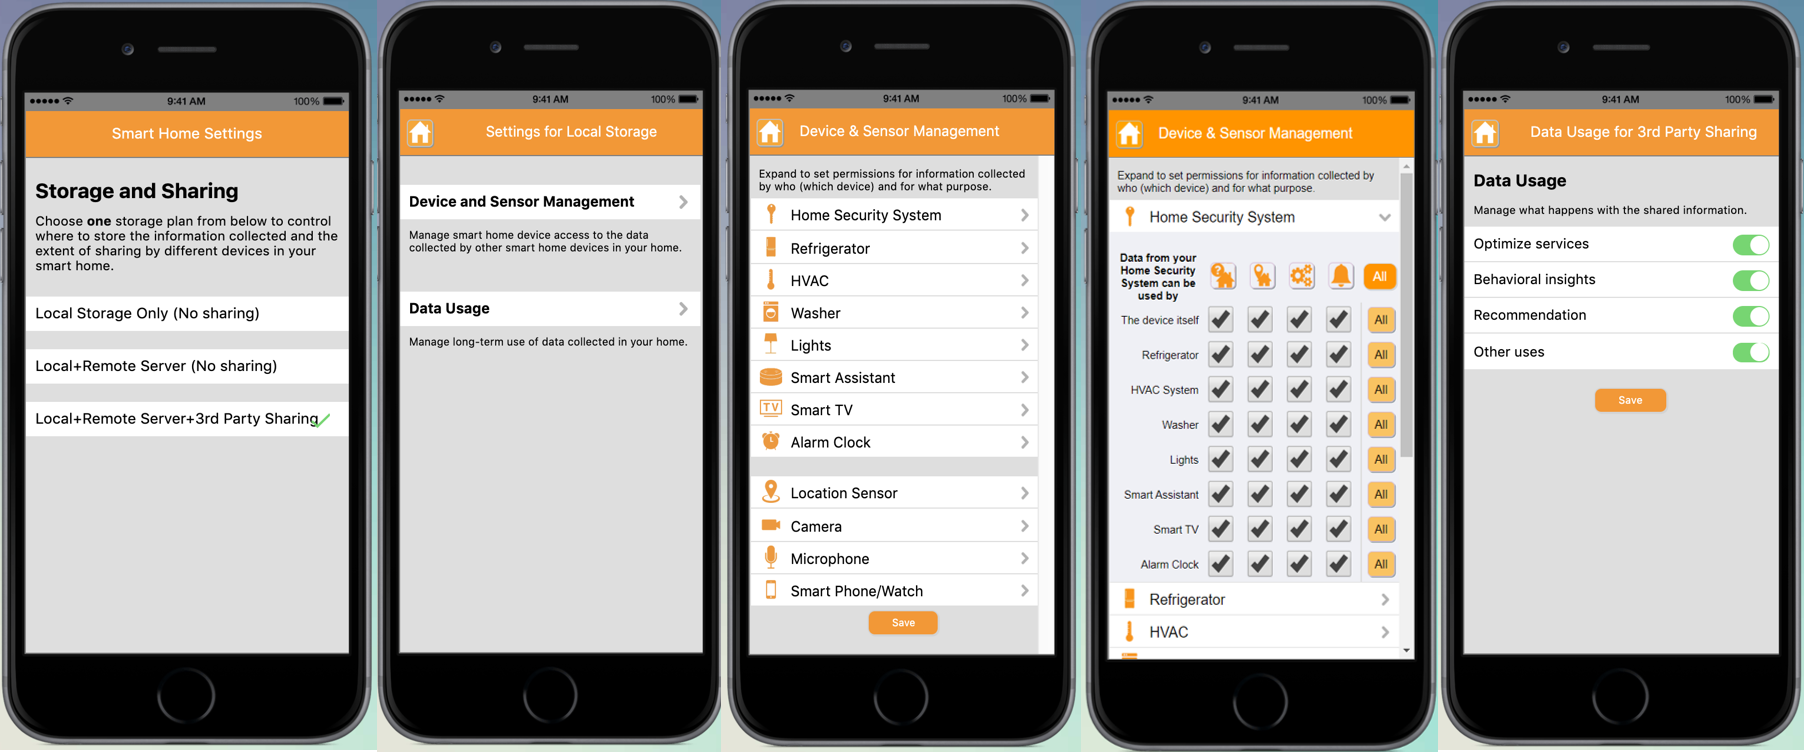
\includegraphics[width=\textwidth]{figures/ui2AllOn.png}
	\caption{User Interface 2 with all settings turned on}
	\label{fig:ui2AllOn}
\end{figure}

%Figure~\ref{fig:ui1OneR} shows the experimental condition --- UI1:Smart Default.
\begin{figure}
	\centering
	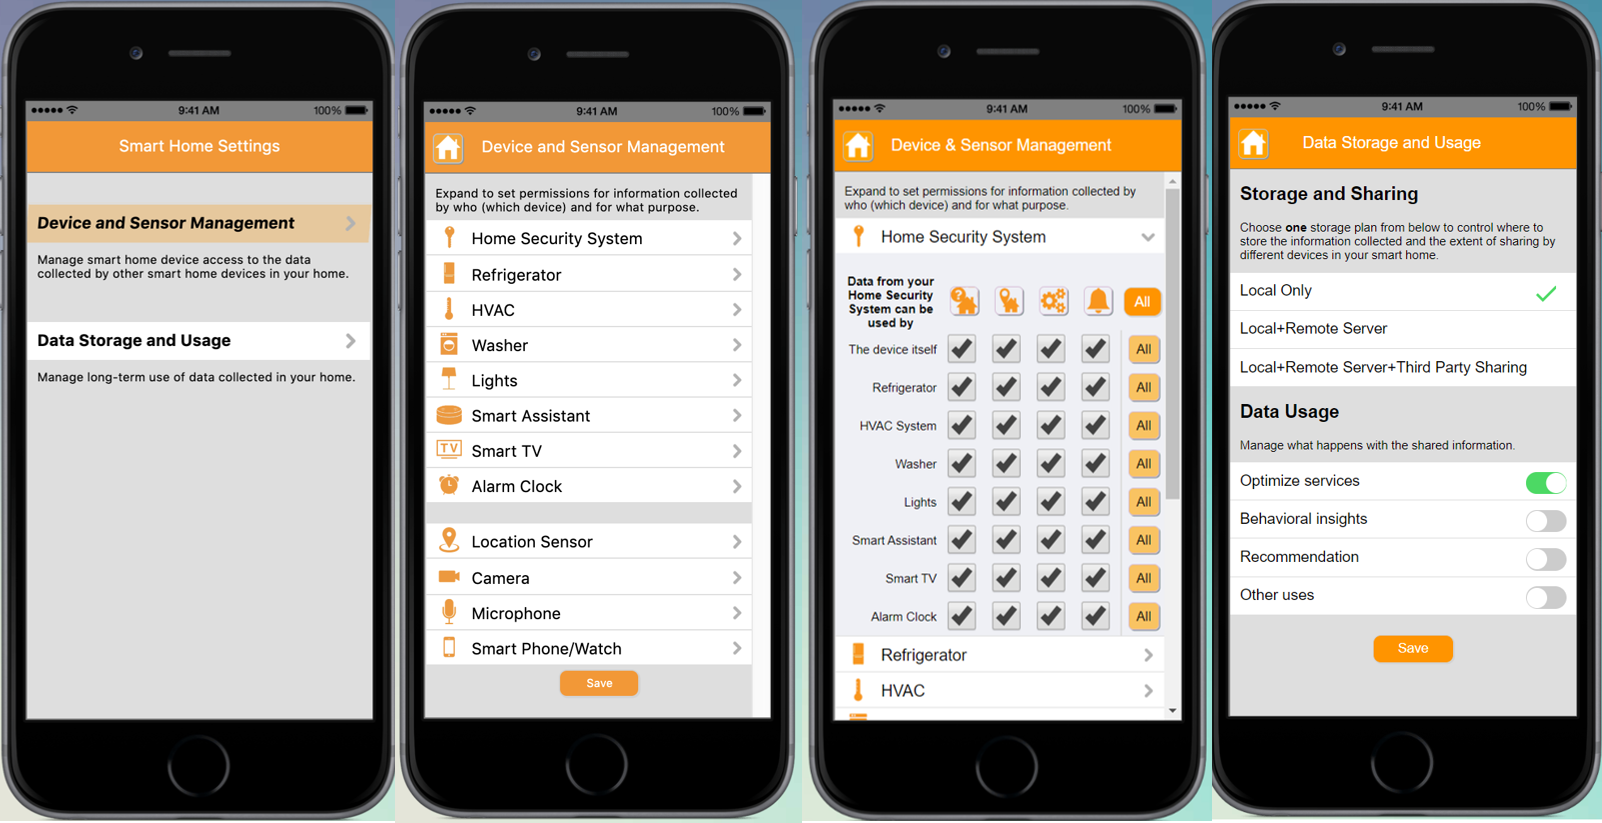
\includegraphics[width=\textwidth]{figures/ui1OneR.png}
	\caption{User Interface 1 with Smart Default}
	\label{fig:ui1OneR}
\end{figure}

%Figure~\ref{fig:ui2SD} shows the experimental condition --- UI2:Smart Default.
\begin{figure}
	\centering
	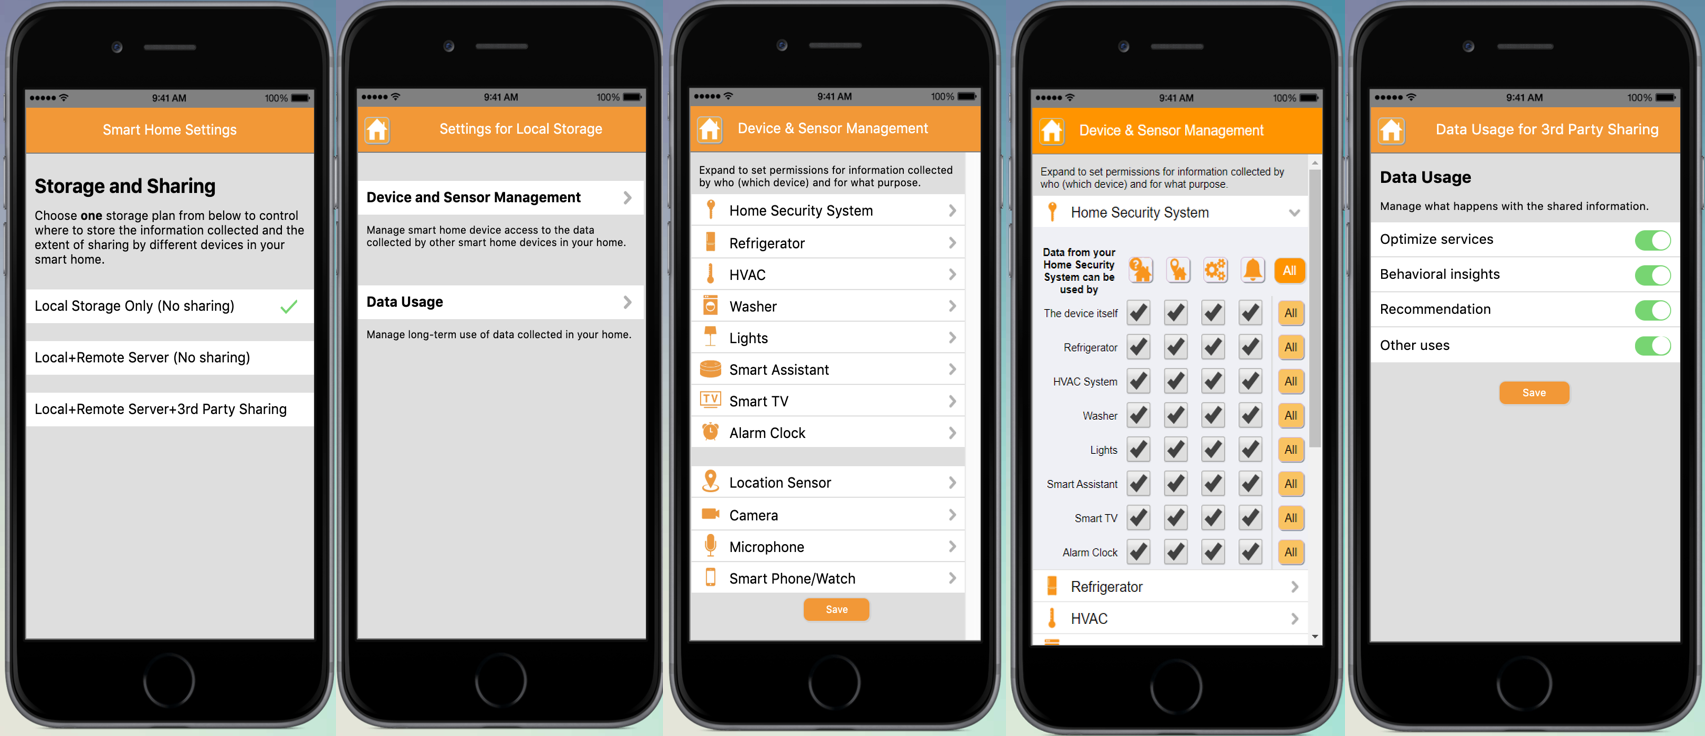
\includegraphics[width=\textwidth]{figures/ui2SD.png}
	\caption{User Interface 2 with Smart Default}
	\label{fig:ui2SD}
\end{figure}

%Figure~\ref{fig:ui1Profiles} shows the experimental condition --- UI1:Smart Profiles.
\begin{figure}[htb]
	\centering
	\begin{subfigure}[t]{0.2\textwidth}
		\centering
		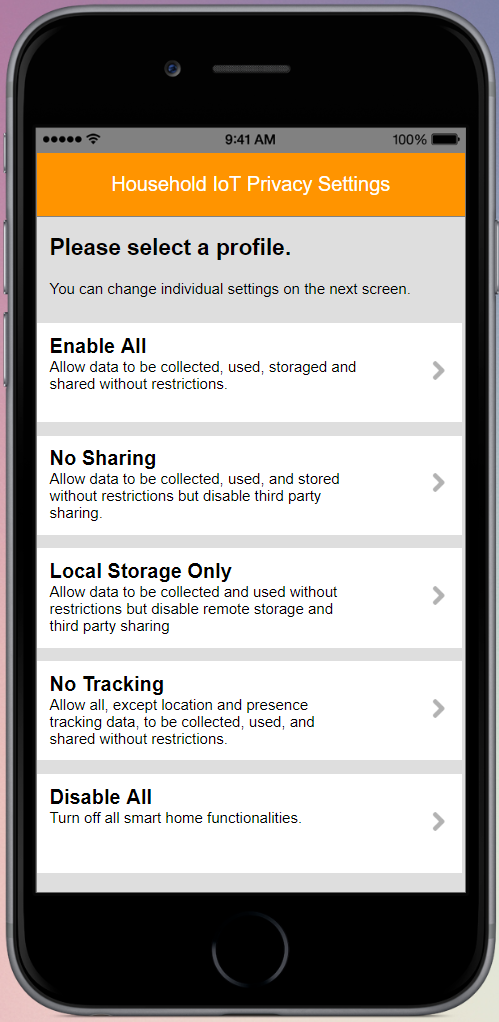
\includegraphics[height=2.8in]{figures/ui1sp1.png}
	\end{subfigure}%
	~~~~~
	\begin{subfigure}[t]{0.2\textwidth}
		\centering
		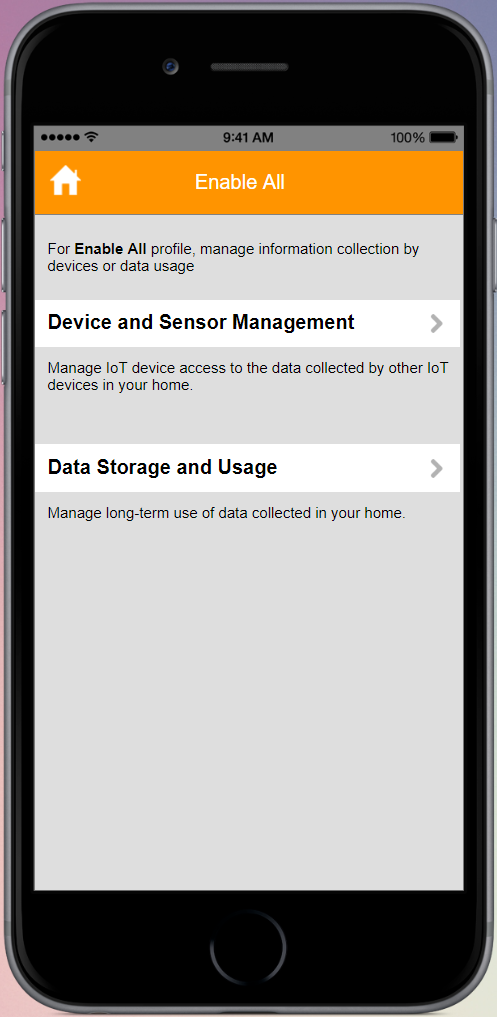
\includegraphics[height=2.8in]{figures/ui1sp2.png}
	\end{subfigure}%
	~~~~~
	\begin{subfigure}[t]{0.2\textwidth}
		\centering
		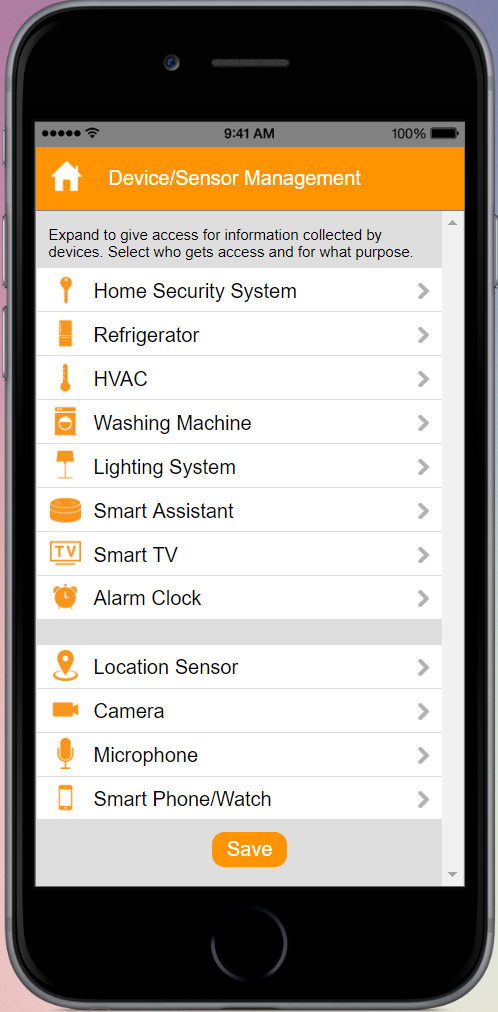
\includegraphics[height=2.8in]{figures/ui1sp3.png}
	\end{subfigure}%
	~~~~~
	\begin{subfigure}[t]{0.2\textwidth}
		\centering
		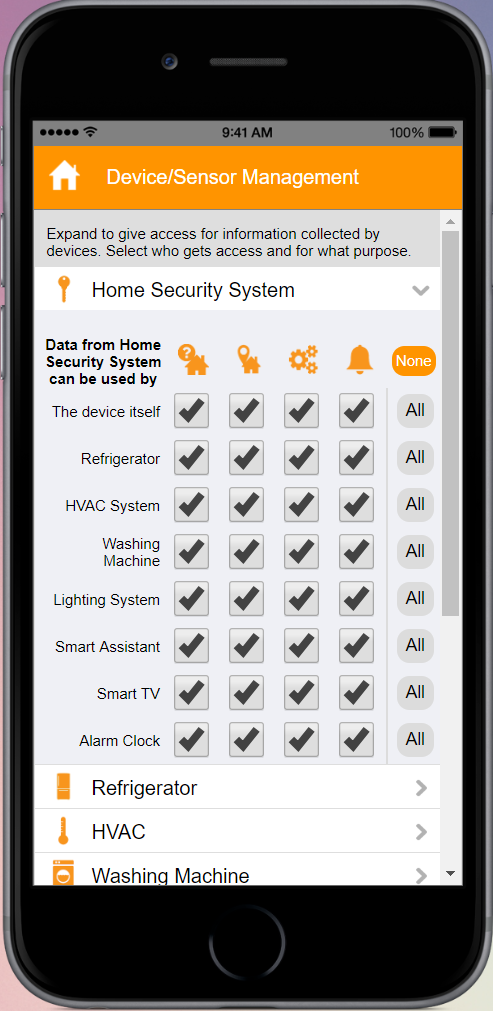
\includegraphics[height=2.8in]{figures/ui1sp4.png}
	\end{subfigure}%
	~~~~~
	\begin{subfigure}[t]{0.2\textwidth}
		\centering
		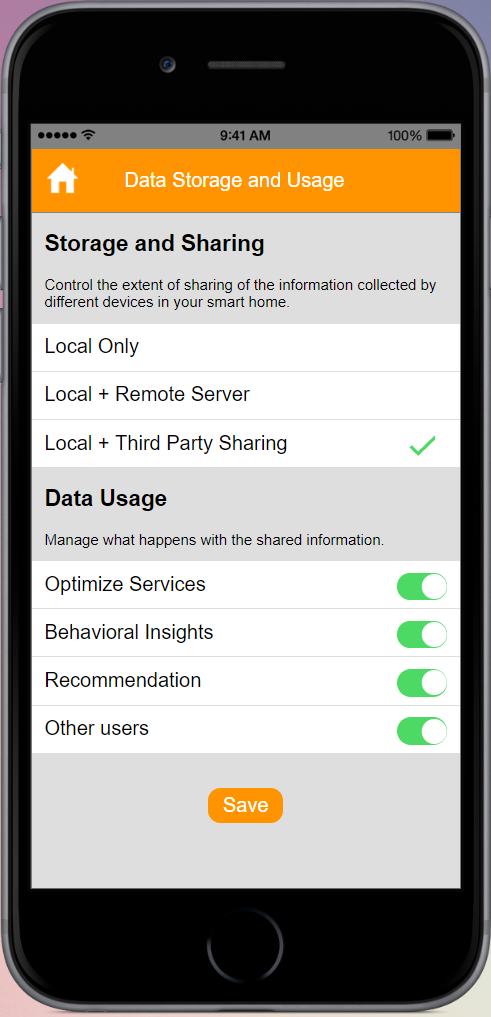
\includegraphics[height=2.8in]{figures/ui1sp5.png}
	\end{subfigure}%
	\caption{User Interface 1 with Smart Profiles}
	\label{fig:ui1Profiles}
\end{figure}

%Figure~\ref{fig:ui2Profiles} shows the experimental condition --- UI2:Smart Profiles.
\begin{figure}[htb]
	\centering
	\begin{subfigure}[t]{0.2\textwidth}
		\centering
		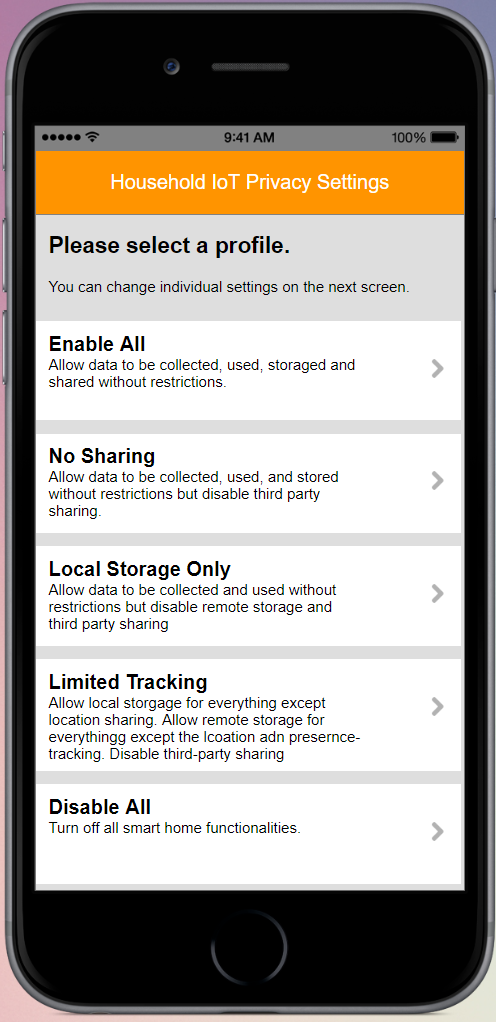
\includegraphics[height=2.8in]{figures/ui2sp1.png}
	\end{subfigure}%
	~~~~~
	\begin{subfigure}[t]{0.2\textwidth}
		\centering
		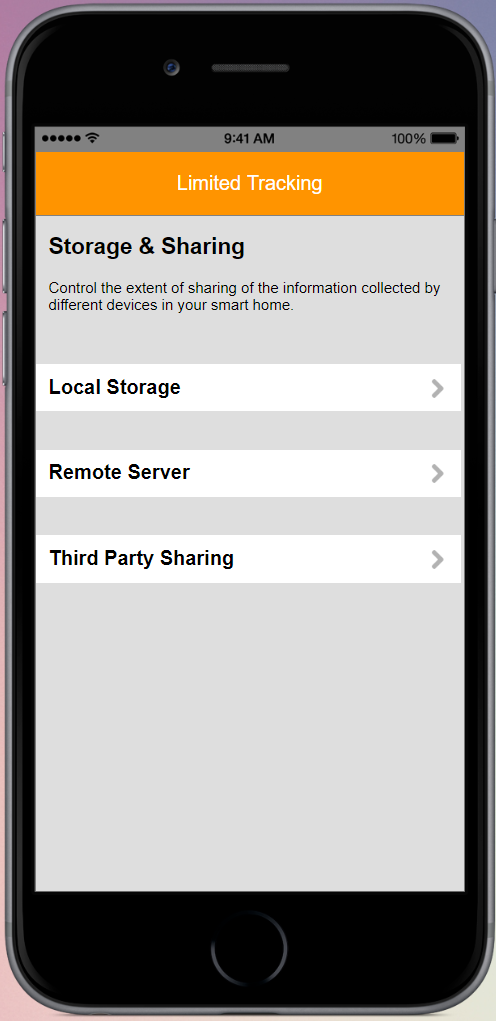
\includegraphics[height=2.8in]{figures/ui2sp2.png}
	\end{subfigure}%
	~~~~~
	\begin{subfigure}[t]{0.2\textwidth}
		\centering
		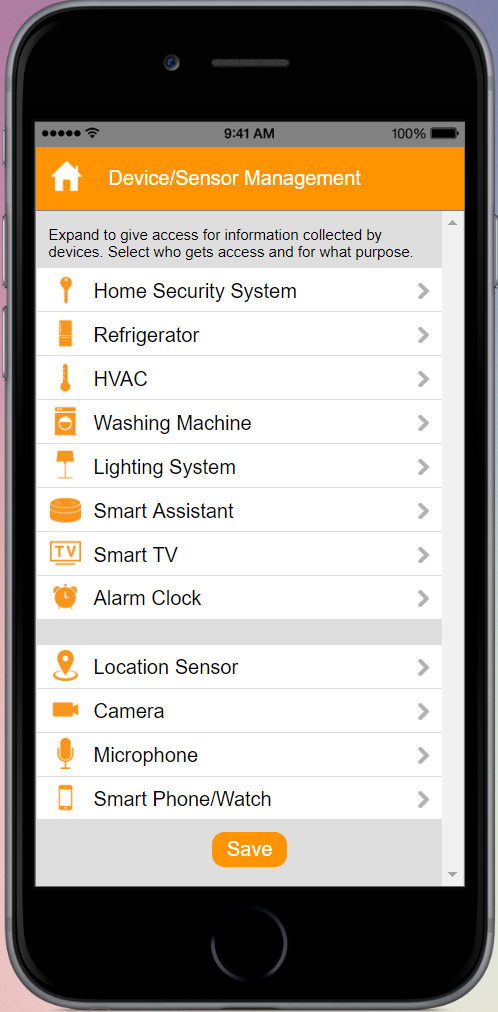
\includegraphics[height=2.8in]{figures/ui1sp3.png}
	\end{subfigure}%
	~~~~~
	\begin{subfigure}[t]{0.2\textwidth}
		\centering
		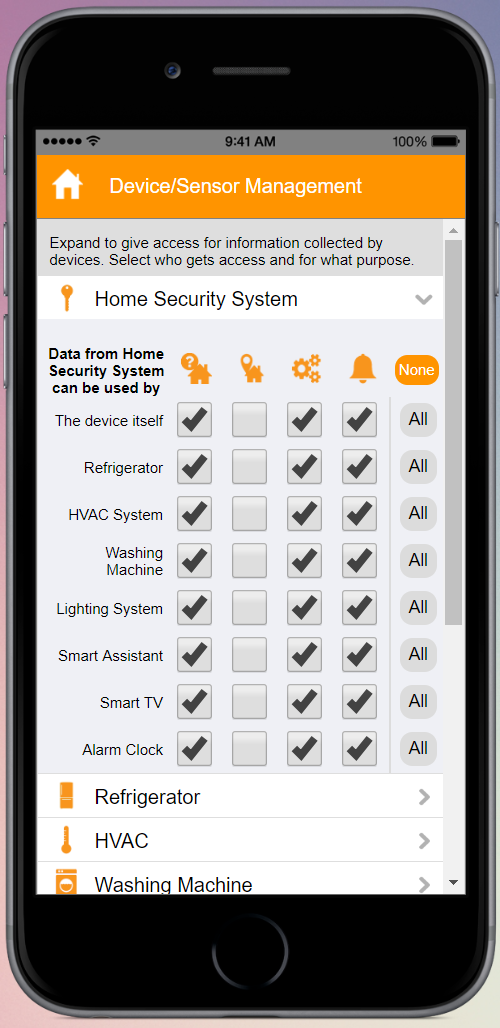
\includegraphics[height=2.8in]{figures/ui2sp4.png}
	\end{subfigure}%
	~~~~~
	\begin{subfigure}[t]{0.2\textwidth}
		\centering
		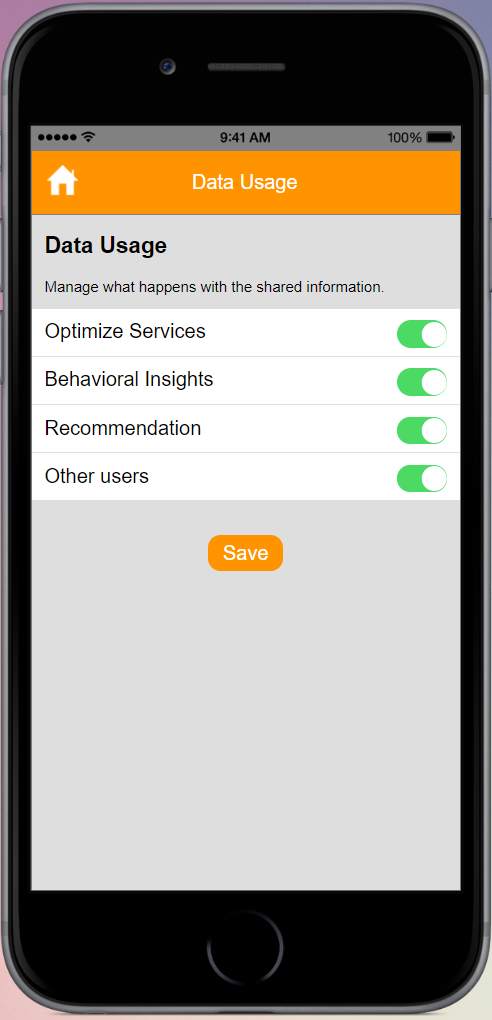
\includegraphics[height=2.8in]{figures/ui2sp5.png}
	\end{subfigure}%
	\caption{User Interface 2 with Smart Profiles}
	\label{fig:ui2Profiles}
\end{figure}
